%% SOURCE: experiments/010-kuzmin-tmi/scripts/inference_4_panel_design.py -- axis from results/inference_4/engineering_axis_genes.csv, strata from engineering_strata.csv, candidates from panel20_candidates.csv, designs from panel20_designs.csv, the panel from panel20_triples.csv and panel20_strains.csv, gene support from gene_candidates.csv, counts from panel20_summary.json; rescue split from inference_4_panel_rescue_decomposition.py (panel20_rescue_decomposition.{csv,json}); scoring from inference_4_panel_score.py; overlap from inference_4_panel_overlap.py; split-labeled agreement from inference_4_measured_diagnostic.py; test-split calibration from calibration_on_test_split.py (results/test_split_calibration.{csv,json})

\section{A 20-strain panel\secstatus{todo}}\label{sec:panel20}

\subsection{What 20 strains buys, exactly\secstatus{todo}}

Wild type sits on every plate as the normalizer and is not a build, so the budget
is 20 constructed genotypes. Closing $\tau$ on a set of triples costs
\[
  \text{strains} \;=\; |\text{genes}| + |\text{doubles}| + |\text{triples}|,
\]
because each triple needs all three of its singles and all three of its doubles
measured beside it. A complete block on $k$ genes therefore costs
$k + \binom{k}{2} + \binom{k}{3}$: 7 strains at $k = 3$, 14 at $k = 4$, and 25 at
$k = 5$. So the complete five-gene block that carried the previous design does not
fit, and the complete four-gene block leaves 6 strains idle while closing only 4
interactions. The shape has to be derived rather than assumed.

\begin{proposition}
Within 20 constructed strains, at most 6 trigenic interactions can be closed, and
6 is reached only on 5 genes with 9 of the 10 doubles built.
\end{proposition}

\begin{proof}
\pfstep{Read the design as a graph} Let the genes be vertices and the built
doubles edges. Every closed triple is a triangle whose three edges are built, so
a design on $g$ genes with $P$ edges and $t$ triangles costs $g + P + t \le 20$.
A gene is built only if some triple contains it, so every vertex lies in a
triangle and carries degree $d_v \ge 2$, which gives $P \ge g$.

\pfstep{Count paths of length two} A vertex of degree $d_v$ is the center of
$\binom{d_v}{2}$ such paths, and every triangle contains exactly three of them,
one centered at each of its vertices. Hence
\[
  3t \;\le\; \sum_{v} \binom{d_v}{2}, \qquad \sum_{v} d_v = 2P .
\]
The summand is convex, so for a fixed degree sum the right side is largest when
the degrees are as unequal as the constraints $2 \le d_v \le g-1$ allow. That is
the only tool the rest of the proof needs.

\pfstep{At most four genes} Only $\binom{4}{3} = 4$ triples exist, so $t \le 4$.

\pfstep{Five genes} Suppose $t = 7$. The budget leaves $P \le 8$, so
$\sum_v d_v \le 16$ over five vertices with $2 \le d_v \le 4$, and the extreme
allocation $(4,4,4,2,2)$ gives $\sum_v \binom{d_v}{2} = 20$. Then $3t \le 20$
forces $t \le 6$, a contradiction. So $t \le 6$ at five genes.

\pfstep{Six is attained, and only with nine doubles} $K_5$ minus one edge has 9
edges and 7 triangles, and closing 6 of them costs $5 + 9 + 6 = 20$. Eight edges
do not suffice: $K_5$ minus two edges has 5 triangles when the removed pair
shares a vertex and 4 when it does not, both below 6. So $P = 9$ is forced.

\pfstep{Six genes} Suppose $t = 6$. The budget leaves $P \le 8$, so
$\sum_v d_v \le 16$ over six vertices with $d_v \ge 2$, and the extreme
allocation $(5,3,2,2,2,2)$ gives $\sum_v \binom{d_v}{2} = 17$. Then
$3t \le 17$ forces $t \le 5$, a contradiction.

\pfstep{Seven genes} Suppose $t = 6$. The budget leaves $P \le 7$, so
$\sum_v d_v \le 14$; but seven vertices of degree at least 2 already sum to 14,
so every degree is exactly 2 and the graph is a disjoint union of cycles. Seven
vertices hold at most two disjoint 3-cycles, so $t \le 2$.

\pfstep{Eight genes or more} $t = 6$ leaves $P \le 6$, while $P \ge g \ge 8$.
\end{proof}

The optimum is therefore 5 genes, 9 doubles, 6 triples, and the one double left
unbuilt decides which three triples are given up.

\subsection{The engineering axis, and where it reaches\secstatus{todo}}

The axis is the roster restricted to the four central-carbon areas the
strain-design survey names, taken through yeast-GEM 9.0.2 subsystem membership
rather than by hand: glycolysis and gluconeogenesis, the pentose phosphate
pathway, the citric acid cycle, and pyruvate metabolism. That is 84 of the 934
roster genes, and it recovers the loci a reader would expect, among them
\gene{PDC1}, \gene{PDC5}, \gene{PDC6}, \gene{ADH1}, \gene{ADH2}, \gene{ALD4},
\gene{ALD6}, \gene{PYC1}, \gene{PYC2}, \gene{PCK1}, \gene{TAL1}, \gene{TKL1},
\gene{RPE1} and \gene{GRE3}.

Membership in a pathway is not the same as being a validated intervention, and
the axis carries genes no campaign has deleted. It is a reproducible proxy for
the survey's pathway-level claim, not a curated target list.

A triple can hold at most two axis genes, because the space requires at least one
regulator. So the two-axis stratum is the engineering-loaded extreme rather than
a middle case.

\subsection{The model's strong predictions avoid the engineering axis\secstatus{todo}}

This is the finding that constrains everything below, and it runs against the
panel's interest rather than for it.

\begin{table}[H]
\centering
\footnotesize
\begin{tabular}{lrrrrrr}
\toprule
Axis genes & Triples & Share & $>+0.08$ & $>+0.12$ & $>+0.16$ & $>+0.30$ \\
\midrule
0 & 33{,}318{,}318 & 79.6\% & 2{,}255 & 686 & 349 & 120 \\
1 &  8{,}094{,}624 & 19.3\% &   623 & 142 &  82 &  32 \\
2 &    464{,}290 &  1.11\% &    \textbf{28} &   \textbf{3} &   \textbf{1} &   \textbf{0} \\
\bottomrule
\end{tabular}
\caption{Consensus-positive triples by how many engineering-axis genes they
carry, over the 41{,}877{,}232-triple space. Columns count triples every one of
the three checkpoints puts above the cut, so the rows sum to the 2{,}906 / 831 /
432 / 152 of the ranking figure. Generated by
\protect\file{experiments/010-kuzmin-tmi/scripts/inference_4_panel_design.py}.}
\end{table}

The two-axis stratum is 1.11 percent of the space and holds 0.96 percent of the
ordinary consensus tier, which is proportional. It then falls away as the cut
rises: 0.36 percent at $+0.12$, 0.23 percent at $+0.16$, and none at all above
$+0.20$. Its best consensus prediction is $+0.164$, against $+2.08$ for the
axis-free stratum. The one-axis stratum tracks its share at every cut, so the
depletion is specific to triples carrying two.

That reproduces on a sharper axis what the previous space showed for metabolic
content, where no all-metabolic triple cleared the call anywhere. Two readings
remain open and these counts separate neither: the combinations may genuinely
carry less three-way effect, or the model may have learned less about them.

\subsection{The choice this forces\secstatus{todo}}

A panel drawn from the strong consensus tier would be built on \gene{CTI6},
\gene{KRE2}, \gene{CUP9} and \gene{KTR6}, the four genes carrying most of the top
500, and only \gene{CUP9} of those is a regulator the axis would ever pair with
metabolism. A panel drawn from the engineering axis is built on the loci
campaigns return to, and buys that with predictions in the ordinary tier rather
than the strong one. The two cannot be had together in this space, and this
panel takes the second.

\subsection{The chassis pair is the pyruvate node\secstatus{todo}}

Requiring every checkpoint above $+0.08$ and two axis genes leaves 28 triples.
\gene{PDC1} carries 22 of them and \gene{LAT1} 9, and the axis pair co-occurring
most often is \gene{PDC1} with \gene{LAT1}, in 4. Ties on co-occurrence are broken
by screen support, which is decisive here: \gene{PDC1} and \gene{LAT1} were
measured under 608 distinct Kuzmin query screens between them, against 309 for the
next pair, \gene{PDX1} with \gene{LAT1}.

The pair is also the one the survey points at, and yeast-GEM says so directly:
\gene{PDC1} carries \texttt{r\_0959}, pyruvate decarboxylase, the fermentative
exit to acetaldehyde, and \gene{LAT1} carries \texttt{r\_0961}, pyruvate
dehydrogenase, the exit to acetyl-CoA. They are the two reactions that consume
pyruvate, so deleting both restricts exactly the branch point the survey names
first. \gene{PDX1} shares \texttt{r\_0961} with \gene{LAT1}, which is why the two
compete for the same slot.

The growth cost of the pair is already published: the double measures $0.8593$
with $\varepsilon = -0.0273$ in Costanzo 2016 at 30~C, against singles of
$0.9695$ and $0.9145$.

The overlap with the ranked head is thin and worth stating beside this. Of the 79
genes carrying the top 500, 3 are on the axis, $3.8$ percent against the roster's
$9.0$ percent: \gene{LAT1} in 80 of the top 500, \gene{PDX1} in 19, and
\gene{PDC1} in 1. The model's favorite genes are largely not the ones campaigns
delete, and \gene{LAT1} is the exception carrying almost all of the overlap.

\subsection{The panel\secstatus{todo}}

Five genes, nine doubles, six triples, 20 strains. The unbuilt double is
\gene{CAD1} with \gene{CUP9}, which gives up the three triples containing both
and leaves seven closable. The budget pays for six, so one more is given up:
\gene{TOS8} \gene{PDC1} \gene{CUP9}, predicted $+0.097$ on its worst checkpoint.
Two genes are the chassis and three are regulators: \gene{CAD1} and \gene{CUP9}
appear in both TFLink and the SGD regulatory graph, \gene{TOS8} in TFLink only.

\pfstep{The objective cannot choose which seventh to drop, and that matters}
Designs are ranked on the median of their six worst-checkpoint scores, and a
median over six is fixed by the third and fourth entries. Dropping any of the
three weakest triples therefore returns the same median of $+0.128$ at the same
20 strains, so three distinct panels tie for the optimum and the search takes
whichever it reaches first. They do not tie on their floor. Dropping
\gene{CAD1} \gene{TOS8} \gene{LAT1} instead would leave a weakest member of
$+0.081$ rather than $+0.020$. This is the same class of defect as the previous
round, where an objective with no tiebreak let one gene take the panel, and it is
recorded here as a decision still open rather than as a property of the shape.

\begin{table}[H]
\centering
\footnotesize
\begin{tabular}{llrrrr}
\toprule
Gene & Role & Fitness & Screens & Trigenic records & Top-500 triples \\
\midrule
\gene{PDC1} & chassis, glycolysis   & 0.9695 & 309 & 319 & 1 \\
\gene{LAT1} & chassis, glycolysis   & 0.9145 & 299 & 309 & 80 \\
\gene{CAD1} & regulator             & 0.9979 & 10  & 1{,}050 & 2 \\
\gene{TOS8} & regulator             & 1.0204 & 11  & 1{,}074 & 44 \\
\gene{CUP9} & regulator             & 0.9402 & 11  & 1{,}074 & 99 \\
\bottomrule
\end{tabular}
\caption{The five panel genes. Every one is within 9 percent of wild type on its
own, so no triple is built on a sick single. The two support columns disagree by
design and both matter: the regulators fail the 50-screen gate the roster used,
yet each carries over a thousand trigenic training records, well above the
200-record floor the previous panel applied. Subsystem membership is yeast-GEM
9.0.2; fitness is the measured single-mutant value from
\protect\file{panel20_strains.csv}. Screen and record counts are the
\texttt{inference\_4} roster's own, from \protect\file{gene_candidates.csv}, and
run one higher for three of these genes than the earlier screen audit quoted in
Section~\ref{sec:screens}, which counts a gene's records on a slightly different
basis.}
\end{table}

\begin{table}[H]
\centering
\footnotesize
\begin{tabular}{llrrrr}
\toprule
Triple & Arm & Worst & Range across checkpoints & Expected $f$ & Predicted $f$ \\
\midrule
\gene{TOS8} \gene{LAT1} \gene{CUP9} & one chassis  & $+0.229$ & $+0.229$ to $+0.711$ & 0.864 & 1.093 \\
\gene{PDC1} \gene{LAT1} \gene{CUP9} & chassis pair & $+0.164$ & $+0.164$ to $+0.331$ & 0.941 & 1.105 \\
\gene{CAD1} \gene{PDC1} \gene{LAT1} & chassis pair & $+0.130$ & $+0.130$ to $+0.340$ & 0.903 & 1.033 \\
\gene{TOS8} \gene{PDC1} \gene{LAT1} & chassis pair & $+0.126$ & $+0.126$ to $+0.232$ & 0.763 & 0.889 \\
\gene{CAD1} \gene{TOS8} \gene{PDC1} & one chassis  & $+0.081$ & $+0.081$ to $+0.368$ & 0.894 & 0.975 \\
\gene{CAD1} \gene{TOS8} \gene{LAT1} & one chassis  & $+0.020$ & $+0.020$ to $+0.151$ & 0.908 & 0.928 \\
\bottomrule
\end{tabular}
\caption{The panel, triple by triple. ``Worst'' is the lowest of the three
checkpoints and is what the design was ranked on. ``Expected $f$'' is the
multiplicative trigenic expectation
$f_{ab}f_c + f_{ac}f_b + f_{bc}f_a - 2f_af_bf_c$ built entirely from published
singles and doubles; ``Predicted $f$'' adds the worst-checkpoint $\tau$ to it.
Generated by
\protect\file{experiments/010-kuzmin-tmi/scripts/inference_4_panel_design.py}.}
\end{table}

\begin{figure}[H]
\centering
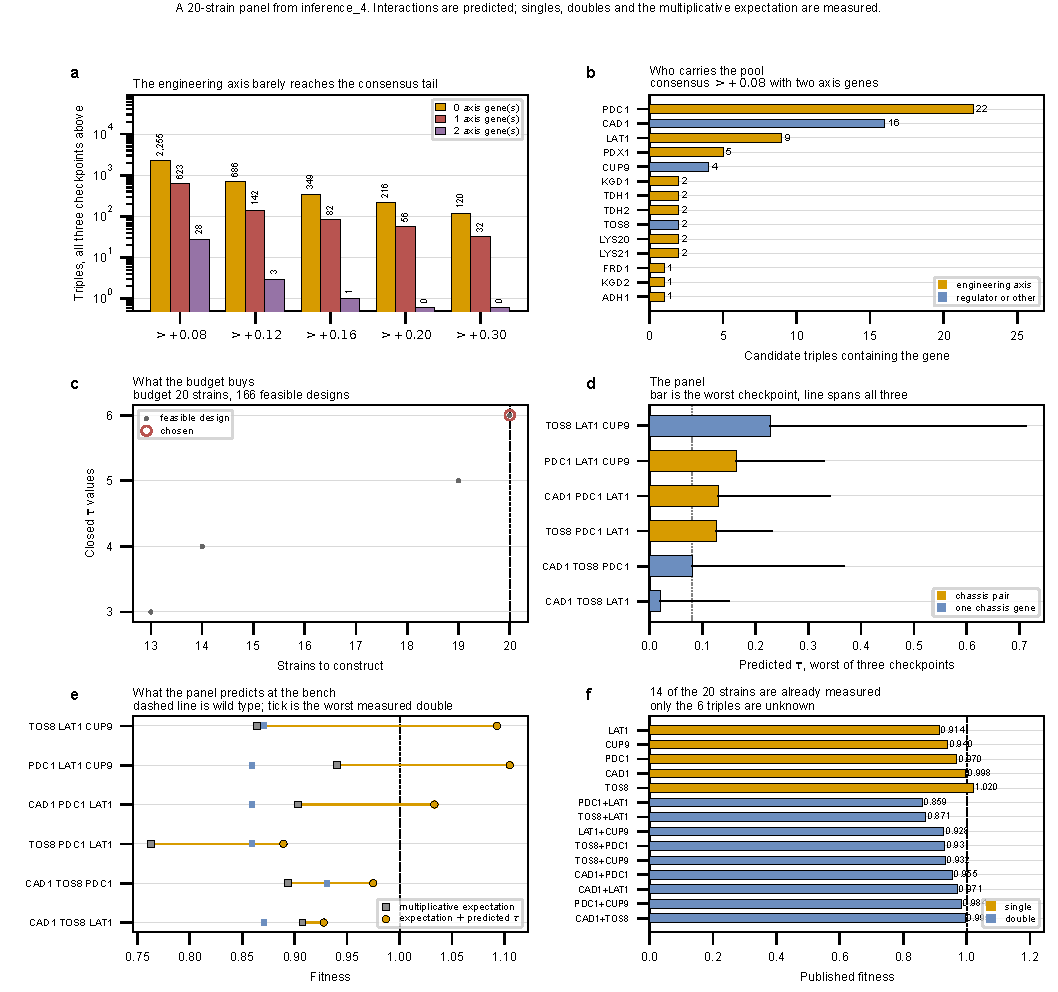
\includegraphics[width=\linewidth]{figures/inference_4_panel_design.pdf}
\caption{\textbf{a}, consensus-positive triples by engineering-axis content, with
counts labeled including the zeros. \textbf{b}, the genes carrying the candidate
pool, colored by axis membership. \textbf{c}, closed $\tau$ against strains for
every feasible design, with the 20-strain budget marked. \textbf{d}, the panel's
predicted interactions, bar at the worst checkpoint and line spanning all three,
colored by arm. \textbf{e}, the measured multiplicative expectation of each
triple and where the predicted $\tau$ places it, against wild type and against
the triple's worst measured double. \textbf{f}, the 14 panel strains that already
carry published fitness. Generated by
\protect\file{experiments/010-kuzmin-tmi/scripts/inference_4_panel_design.py}.}
\end{figure}

\subsection{The rescue ordering is the readable experiment\secstatus{todo}}

The three chassis-pair triples share their first two deletions, so their
expectations differ only through the third gene and the comparison is
within-chassis. Against the measured chassis double at $0.8593$, the predicted
recoveries are $+0.246$ for \gene{CUP9}, $+0.174$ for \gene{CAD1} and $+0.030$
for \gene{TOS8}.

That ordering is the claim to test, and it is testable independently of whether
the magnitudes are right, but not for the reason it first appears. Split each
recovery into the part built from published fitness and the part the model
supplies,
\[
  f_{abc} - f_{ab} \;=\; \underbrace{(f_{ac}f_b + f_{bc}f_a - 2f_af_bf_c
  + f_{ab}f_c - f_{ab})}_{\text{measured}} \;+\; \tau_{abc}.
\]
The measured offsets are $+0.081$, $+0.044$ and $-0.096$, a spread of $0.178$.
The three predicted $\tau$ are $+0.164$, $+0.130$ and $+0.126$, a spread of
$0.038$. So the published lower rungs alone already order the three regulators,
and they contribute $82$ percent of the separation.

Two things follow, and they pull opposite ways. The ordering is robust: shrinking
$\tau$ by any factor $s \ge 0$ leaves both gaps positive, since
$0.038 + 0.034s > 0$ and $0.140 + 0.004s > 0$, so no amount of the miscalibration
established below can flip it. And the ordering is a weak test of the model,
because it would come out the same if the model contributed nothing at all.
Reading the panel as a check on the transformer requires the arm contrast and the
magnitudes, not this ranking.

The panel answers a second question at the same time. The highest prediction in
the whole pool, \gene{TOS8} \gene{LAT1} \gene{CUP9} at $+0.229$, carries only one
chassis gene, so the model does not say both pyruvate exits must be blocked. If
measurement puts the three chassis-pair triples above the one-chassis triples, the
prediction is about the branch point. If it does not, the effect belongs to the
regulators. That leading entry turns out to be a training record with a measured
$\tau$ of $+0.228$, set out below, so it enters the comparison as a control rather
than as a test.

\gene{CAD1} \gene{TOS8} \gene{LAT1} at $+0.020$ is a near-null member and serves
as the internal control. It is there by a tie rather than by necessity: as set
out above, an equally optimal design drops it and keeps \gene{TOS8} \gene{PDC1}
\gene{CUP9} at $+0.097$ instead. Keeping the near-null member is defensible,
since a panel of six uniformly positive predictions has no interior point that
the model expects to measure flat, but it should be kept on that argument rather
than on the shape.

One check on the ordering, against the single-gene scores reported later in this
section. Ranked on their own the three regulators go \gene{TOS8} $+0.0532$,
\gene{CUP9} $+0.0389$, \gene{CAD1} $+0.0171$; ranked by predicted recovery they go
\gene{CUP9}, \gene{CAD1}, \gene{TOS8}. The two orderings disagree, and \gene{TOS8}
is the extreme case, carrying the largest single-gene score and the smallest
predicted rescue. So this particular ranking is not a restatement of the per-gene
scores, which is the one piece of evidence the panel has on that question before
it is built.

\subsection{Where the magnitudes stop being credible\secstatus{todo}}

Two of the six predicted triple fitnesses land above wild type, at $1.105$ and
$1.093$. The genome-wide deletion ceiling is $1.1118$, only $2.7$ percent of
single deletions are significantly above wild type, and in Kuzmin the fraction of
strains above wild type falls with order, $23.0$ to $13.8$ to $6.9$ percent. So
these two levels sit at the extreme of everything ever measured on a deletion
strain, and they should be read as the ranking saturating rather than as a
forecast.

The widest checkpoint disagreement sits on the leader: \gene{TOS8} \gene{LAT1}
\gene{CUP9} spans $+0.229$ to $+0.711$, a factor of three. Its rank is carried by
the checkpoint that likes it least, which is why the worst-checkpoint statistic
was used, but the spread is still the largest in the panel.

\subsection{Two tests that cost no strains\secstatus{todo}}

\pfstep{Score the free-fatty-acid panel with the same model} That screen already
has the structure this panel is being built to create, a flux chassis crossed
against regulator deletions, and all 720 orders are measured. Asking whether the
transformer's growth $\tau$ predicts the sign or the rank of the measured titer
$\tau$ costs one inference pass and no strains. A null result is informative,
because it separates ``the model ranks growth interactions'' from ``the model
ranks interactions that matter for production'', and nothing currently
distinguishes those two.

\pfstep{Rank the rescue rather than the interaction} For a fixed chassis double
$\{a,b\}$, the same identity gives
$f_{abc} = \tau_{abc} + f_{ab}f_c + f_{ac}f_b + f_{bc}f_a - 2f_af_bf_c$, so
ranking third genes $c$ by predicted $f_{abc} - f_{ab}$ answers the question an
engineer actually asks, which deletion best restores the chassis. The
shrinkage that makes predicted $\tau$ uncalibrated is monotone, so it preserves
the ranking of $\tau$, and the remaining terms are measured rather than
predicted. The ranking therefore uses published fitness where it exists and the
model only where it does not.

\subsection{Fifteen of the twenty strains are already measured\secstatus{todo}}

Five genes admit $\binom{5}{2} = 10$ pairs, of which the design builds 9 and drops
\gene{CAD1} with \gene{CUP9}. Every one of those 9, and every one of the 5
singles, already carries a published fitness: 5 of the 14 from Costanzo 2016 at
30~C and 9 from the Kuzmin screens. A sixth rung turns out to be known as well,
\gene{TOS8} \gene{LAT1} \gene{CUP9}, for the reason set out below, so 15 of the 20
are known and 5 are unknown. Two things follow.

The build is still all 20 strains, because $\tau$ is a difference and a
carried-forward reference costs up to $1.46$ times the standard error, so every
order has to sit on the same plates. What changes is that 15 of the 20 arrive
with a published value attached, which makes them a plate-level calibration set
rather than a cost. The two kinds of prior value are not interchangeable: 14
lower rungs carry a published \emph{fitness}, and the fifteenth is a triple
carrying a published $\tau$, which is a different quantity measured on a
different scale. The previous round could not tell a normalization artifact from
a real effect, and 14 known fitnesses measured beside 6 triples is what would
have caught it: singles reproduced Costanzo at $r = 0.706$ while doubles did not,
at $r = 0.255$, and that diagnosis needed exactly this kind of overlap.

\subsection{The model scored on the fourteen known rungs\secstatus{todo}}

Those fourteen answers are already known, so the model can be asked for them before
anything is built. All twenty strains were scored by all three checkpoints on CPU,
the four GPUs being busy with the 025 training run, and twenty records is a few
minutes of CPU.

\pfstep{The scoring path is verified, not assumed} The six triples are members of
the \texttt{inference\_4} space, so the GPU run already scored them, and the CPU
path has to reproduce those 18 values. It does, to a largest absolute difference of
$0.0012$ on a prediction of $0.58$. Exact equality is not the right bar: the GPU run
scored under autocast and this one is float32, so the residual is reduced-precision
rounding. Two things make the check worth writing down. These checkpoints load with
a warning that \texttt{perturbation\_transform} keys are absent, which is cosmetic
because the checkpoint carries the older attribute names that the current module
keeps as aliases of layer 0, so the tensors are shared. And the difference is far
below the effects reported next.

\pfstep{Singles and doubles are zero-shot} The 010 build is 376{,}732 records and
every one is a 3-gene perturbation, read back from the training LMDB. The model has
one output head and no conditioning on perturbation order, so what it emits for a
1- or 2-gene input is its interaction estimate for that set, compared here against
digenic $\varepsilon = f_{ab} - f_a f_b$, the measured counterpart on a comparable
scale. Nothing below measures in-distribution accuracy.

\begin{table}[H]
\centering
\footnotesize
\begin{tabular}{lrrr}
\toprule
Order & Strains & Mean predicted interaction & Truth \\
\midrule
1, singles & 5 & $+0.0714$ & $0$ by definition \\
2, doubles & 9 & $+0.1369$ & measured $\varepsilon$, 6 of 9 negative \\
3, triples & 6 & $+0.2311$ & unknown, the trained order \\
\bottomrule
\end{tabular}
\caption{Predicted interaction against the number of deleted genes. The mean grows
close to proportionally with the count, which is what a model carrying no notion of
order does when taken below the order it was trained on. Generated by
\protect\file{experiments/010-kuzmin-tmi/scripts/inference\_4\_panel\_score.py}.}
\end{table}

\pfstep{The lower rungs were never selected on prediction} The six triples were
chosen for being consensus-positive, so their sign carries no information. The
singles and the doubles were not chosen at all: they are forced by $\tau$ closure
once the triples are fixed, and no prediction of theirs entered the design. What
follows is therefore about the model rather than about the selection.

\pfstep{Three findings, and they are not favorable} A single gene has no
interaction term, yet the mean prediction on the five singles is $+0.0714$, above
the training-label standard deviation of $0.0633$, and \gene{LAT1} alone scores
$+0.2441$. On the nine doubles the model puts every one above its measured
$\varepsilon$, 9 of 9, a sign test at $p = 0.004$, with a mean signed error of
$+0.138$, and it predicts no negative interaction anywhere although 6 of the 9
measured values are negative. Rank agreement is absent at this size, Spearman
$\rho = +0.200$ at $p = 0.61$.

\pfstep{The measured comparison is not an artifact of mixing screens} The nine
$\varepsilon$ are reconstructed from singles and doubles that do not all come from
the same screen, and mixing normalizations across screens is what flipped a sign in
the \gene{pcl6} census. Three of the nine pairs also carry a published Costanzo
$\varepsilon$, and the reconstruction matches it to within $0.007$ on all three, an
order of magnitude below the model's $+0.138$ mean signed error. The direction of
the error therefore survives the source-mixing objection.

\pfstep{What this does and does not license} It does not measure the triples.
Every number here is out of distribution, and a model can be wrong below its
trained order and right at it. What it does establish is that the output carries no
constraint forcing interaction to vanish at order 1, and that it grows with the
count of deleted genes.

That sharpens the concern the ranked head already raised. \gene{LAT1} alone, at
$+0.2441$, scores above five of the six triples that the panel is built to test,
so ``the model reports a per-gene score summed over the perturbation set'' is now a
concrete null rather than a worry. The arm contrast is what separates it from a
genuine interaction claim, and the analysis plan has to state that null before the
plate is read.

\begin{figure}[H]
\centering
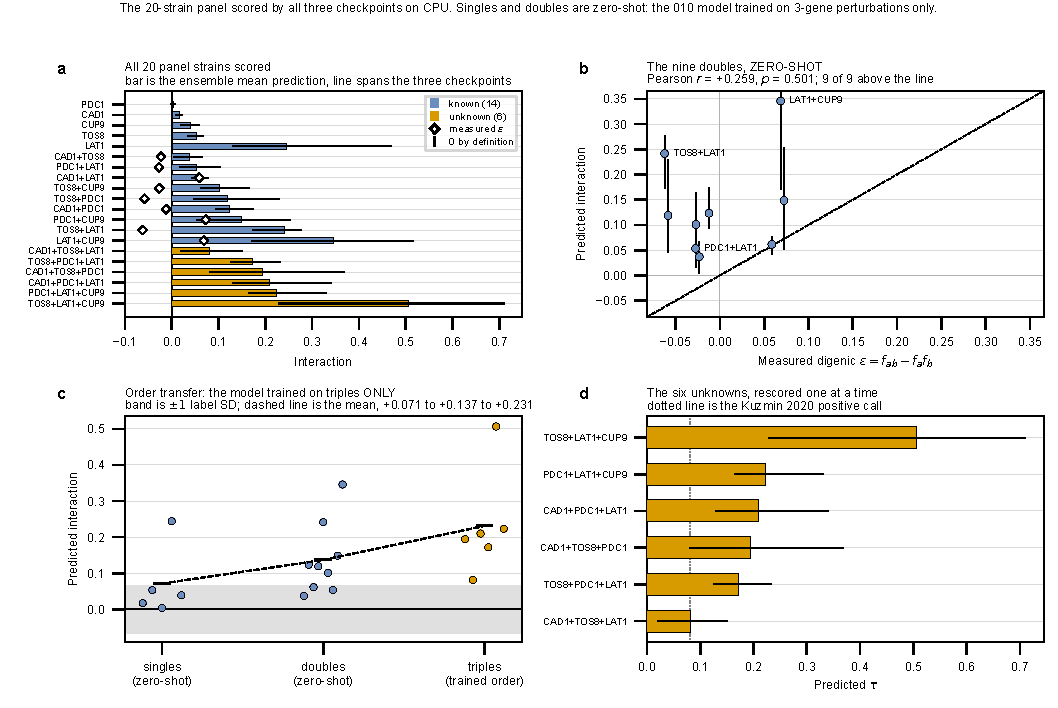
\includegraphics[width=\linewidth]{figures/inference_4_panel_score.pdf}
\caption{\textbf{a}, every panel strain scored, bar at the ensemble mean and line
spanning the three checkpoints, with a diamond where a measured $\varepsilon$
exists and a tick where the interaction is zero by definition. \textbf{b},
predicted against measured on the nine doubles, zero-shot, with the identity line;
every point sits above it. \textbf{c}, prediction against perturbation order, with
the band at $\pm 1$ training-label standard deviation and the dashed line tracking
the mean. \textbf{d}, the six triples, the only strains whose answer is unknown.
Generated by
\protect\file{experiments/010-kuzmin-tmi/scripts/inference\_4\_panel\_score.py}.}
\end{figure}

\subsection{One of the six was already measured, and it is the leader\secstatus{todo}}

The generator enumerates the roster and never removes combinations the Kuzmin
screen already measured, so ``unmeasured space'' was an assumption. It is mostly
right and locally wrong, and the exceptions are worth more than the assumption
was: they are the only triples in this space that carry both a prediction and a
measurement, which is what the next section uses them for.

\pfstep{The space} 4{,}877 of the 41{,}877{,}232 triples, $0.012$ percent, are
already in the 010 build: 3{,}947 in train, 431 in val, 499 in test. Membership is
the sorted gene set, the same identity that carried 010's splits into 025, and the
split is read from 010's own cached assignment rather than recomputed.

\pfstep{The panel} No single or double is in 010, which follows from the build
being 3-gene throughout. One triple is, and it is the highest-scoring member of
the panel. \gene{TOS8} \gene{LAT1} \gene{CUP9} sits in the \emph{training} split
with a measured $\tau$ of $+0.2280$, a called positive. Its worst-checkpoint
prediction is $+0.2286$. The model is reproducing a label it was trained on to
four decimal places, so that entry is recall and not a prediction.

It is also the one panel strain carrying a trained Kuzmin query double,
\gene{TOS8} with \gene{CUP9}, which is why it was in the training data at all:
Kuzmin crosses a query double against an array, so this triple is that screen's
record for array gene \gene{LAT1}.

\pfstep{What to do with it} Keep it, and relabel it. A strain whose $\tau$ is
already known to be $+0.228$ is a positive control that rides the same plate as
the unknowns, which is worth more than the sixth test would have been. The panel
is then \textbf{15 known rungs and 5 unknown triples}, and the arm contrast is
unaffected because the entry sits in the one-chassis arm either way.

\pfstep{This is not a coincidence, and that is the real finding} Ranking on
prediction enriches for what the model trained on, because it fits those points.
Against a base rate of $0.012$ percent:

\begin{table}[H]
\centering
\footnotesize
\begin{tabular}{lrrrr}
\toprule
Rank window & Already in 010 & Share & Enrichment & train / val / test \\
\midrule
top 10  &  0 & 0.0\% & --      & 0 / 0 / 0 \\
top 50  &  1 & 2.0\% & 172$\times$ & 1 / 0 / 0 \\
top 100 &  5 & 5.0\% & 429$\times$ & 4 / 0 / 1 \\
top 500 & 15 & 3.0\% & 258$\times$ & 12 / 0 / 3 \\
\bottomrule
\end{tabular}
\caption{Triples of the ranked head that the 010 build already contains, against a
base rate of 4{,}877 in 41{,}877{,}232. Generated by
\protect\file{experiments/010-kuzmin-tmi/scripts/inference\_4\_panel\_overlap.py}.}
\end{table}

\pfstep{And every one of them is over-predicted} All 15 top-500 triples that carry
a measured $\tau$ are predicted above it, and measured is $0.23$ of predicted on
average. The extremes are the worst: rank 12 is predicted $+1.86$ against a
measured $+0.572$, and rank 500 is predicted $+0.350$ against a measured
$-0.102$.

Selection explains part of that. Taking the top of a 41.9-million ranking selects
for positive error, so the winners overstate by construction whether or not the
model is calibrated. What selection does not explain away is the size, roughly a
fourfold inflation at the operating point this panel is drawn from, and it is the
same direction as the zero-shot over-prediction on the doubles.

\pfstep{Three of the 15 are held out} They sit in 010's test split, predicted
$+0.883$, $+0.384$ and $+0.350$ against measured $+0.258$, $+0.015$ and $-0.102$.
Three points settle nothing on their own. The next subsection widens that sample
from 3 to 930 by leaving the top 500 and using every measured triple in the
space.

\begin{figure}[H]
\centering
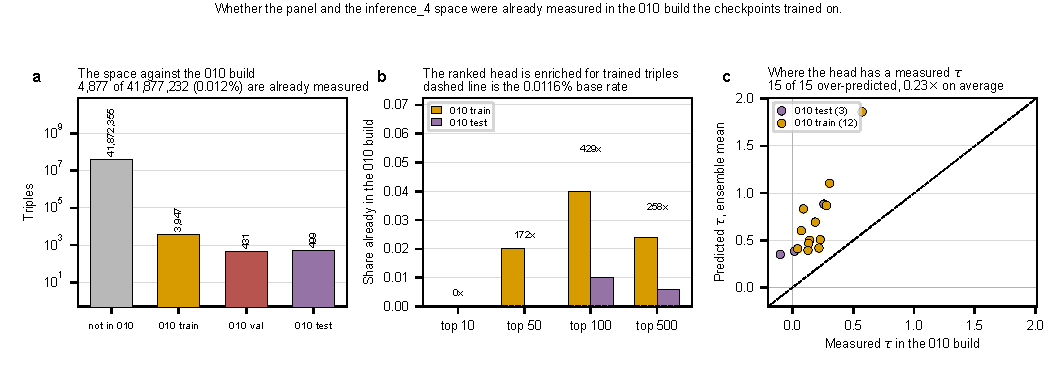
\includegraphics[width=\linewidth]{figures/inference_4_panel_overlap.pdf}
\caption{\textbf{a}, the inference\_4 space against the 010 build the checkpoints
trained on, by split. \textbf{b}, share of each rank window already in that build,
against the base rate over the whole space, labeled with the enrichment.
\textbf{c}, predicted against measured $\tau$ for the 15 triples of the top 500
that carry a measured value, with the identity line; every one sits above it.
Generated by
\protect\file{experiments/010-kuzmin-tmi/scripts/inference\_4\_panel\_overlap.py}.}
\end{figure}

\subsection{The measured overlap as a probe, not a defect\secstatus{todo}}

Dropping the 4{,}877 from the nomination list is one line, and it would throw away
the only triples in this space that carry both a prediction and a measurement.
Labeling them by 010 split instead turns the overlap into the check the space
otherwise cannot run. Train tells you the scoring path works, because the model fit
those. Val and test are held out and are the honest read. The reading is the
contrast between them.

Nothing below needed a GPU or a new inference pass. Predictions for all
41{,}877{,}232 triples already existed, so this is a join.

\begin{table}[H]
\centering
\footnotesize
\begin{tabular}{lrrrr}
\toprule
Subset & $n$ & Pearson $r$ & Calibration slope & Real positives \\
\midrule
train    & 3{,}947 & $+0.417$ & 0.36 & 17 \\
val      &   431 & $+0.073$ & 0.13 &  1 \\
test     &   499 & $+0.258$ & 0.28 &  5 \\
\midrule
held out &   930 & $+0.182$ & 0.24 &  6 \\
pooled   & 4{,}877 & $+0.378$ & 0.35 & 23 \\
\bottomrule
\end{tabular}
\caption{Prediction against measurement for every measured triple in the space.
The slope regresses measured on predicted, so 1 is calibrated and below 1 is
inflation. Real positives are $\tau > +0.08$ at $p < 0.05$. Generated by
\protect\file{experiments/010-kuzmin-tmi/scripts/inference\_4\_measured\_diagnostic.py}.}
\end{table}

\pfstep{Train agrees, so the machinery is sound} $r = +0.417$ over 3{,}947 triples
is in the range of the checkpoints' own validation Pearson of $0.45$ to $0.46$. A
low value here would have meant a broken scoring path rather than biology, and it
is not low.

\pfstep{Held out agrees about half as well} $r = +0.182$ over 930. Val and test
disagree with each other, $+0.073$ against $+0.258$ on similar sample sizes, so
neither is a precise estimate on its own and the pooled value is the one to quote.
The gap between $0.417$ and $0.182$ is the part that matters: the ranking recalls
better than it generalizes, by roughly a factor of two.

\pfstep{Range restriction does not explain the gap} The roster drops essential
genes, sick singles and mitochondrial genes, which compresses the spread of $\tau$
and attenuates any correlation. Measured, that compression is mild: the standard
deviation inside the space is $0.0499$ against $0.0633$ over the whole build, a
ratio of $0.79$. It cannot turn $0.417$ into $0.182$.

\pfstep{The measurements are themselves noisy, which bounds what $r$ can mean}
Only $2.9$ percent of the 4{,}877 measured $\tau$ clear $p < 0.05$, so most of
what the correlation is being scored against is individually indistinguishable
from zero. That attenuates any correlation, which makes $+0.417$ and $+0.182$
floors rather than estimates. It does not rescue the comparison between them,
because both splits are measured the same way, and it does not touch the
calibration slope, since noise in the dependent variable inflates that slope's
standard error without biasing it. The slope is therefore the statistic to argue
from, and the correlations are the ones to hold loosely.

\pfstep{The tail itself cannot be validated, and this is the real limit} Zooming
into the ranking, the top 1{,}000 contains 15 measured triples from train and
\textbf{3} from held out; the top 10{,}000 contains 30 and \textbf{6}. A panel is
drawn from exactly that window, and six points cannot check it. Any statistic
quoted there, in either direction, is noise.

\pfstep{Where it can be checked, the ordering does generalize, on two events}
At the top 100{,}000, where 26 held-out triples finally accumulate, $7.7$ percent
are real positive calls against a held-out base rate of $0.65$ percent, an
enrichment of $11.9\times$. Train over the same window reaches $21.5\times$ on 11
calls of 119. The held-out figure is 2 calls of 26, and the honest statement of
it is a Poisson tail: $0.17$ calls are expected at the base rate and 2 were seen,
$p = 0.013$. That is evidence, and it is thin evidence, and it must be quoted as
2 events rather than as a percentage. Taken with the train comparison the reading
is that the ranking finds real interactions it was never trained on, at roughly
half the rate at which it resurfaces ones it was.

\pfstep{The magnitudes are the weakest part, and they fail on held-out data too}
The pooled calibration slope is $0.35$ and the held-out slope $0.24$, so a
predicted $\tau$ overstates by three to four times. Inside the top 1{,}000 the mean
signed error is $+0.452$ on train and $+0.482$ on test, so this is not a training
artifact. Across the entire predicted range, which spans $-0.8$ to $+1.0$, the mean
measured $\tau$ moves from $-0.02$ to $+0.03$.

\pfstep{This contradicts Section~\ref{sec:positives}, and the contradiction is
the finding} Section~\ref{sec:positives} reports a calibration slope of $0.877$
on the 010 test split and calls
the predictions calibrated. Here the same three checkpoints give $0.24$. Both
numbers are right, and until now neither had a script: the $0.877$ appeared in an
earlier draft with no generating artifact anywhere in the repository, so it could
not be checked. It reproduces exactly, at $0.8769$ over all 37{,}673 test
records.

\begin{table}[H]
\centering
\footnotesize
\begin{tabular}{lrrrr}
\toprule
Population & $n$ & Pearson $r$ & Calibration slope & Mean signed error \\
\midrule
010 test split, all           & 37{,}673 & $+0.478$ & 0.88 & $+0.001$ \\
010 test split, top 100       &      100 & $+0.630$ & 1.59 & $+0.034$ \\
010 test split, top 500       &      500 & $+0.471$ & 1.19 & $+0.018$ \\
\midrule
\texttt{inference\_4}, held out, all  &  930 & $+0.182$ & 0.24 & $+0.022$ \\
\texttt{inference\_4}, held out, top 10{,}000 & 6 & n/a & 0.35 & $+0.332$ \\
\bottomrule
\end{tabular}
\caption{The same checkpoints scored on two populations. Slope regresses measured
on predicted, so 1 is calibrated. Generated by
\protect\file{experiments/010-kuzmin-tmi/scripts/calibration_on_test_split.py} and
\protect\file{experiments/010-kuzmin-tmi/scripts/inference_4_measured_diagnostic.py}.}
\end{table}

Three things separate the populations, and the last one is what should be
carried forward. A whole-split slope is dominated by the bulk near zero, so it
answers a question no panel asks. Inside the head of its own test split the model
does not inflate at all, and the slope runs the other way, $1.59$ at the top 100.
And the head of \texttt{inference\_4} is not the head of the test split: the top
ensemble mean there is $+2.33$, while the largest value these checkpoints ever
emit on labeled data is $+0.63$. The calibration evidence covers a range the
nominated tail leaves entirely.

So the reconciliation is not that one measurement is wrong. It is that
calibration was established on a population that does not include the one the
panel is drawn from, and where the two can be compared the tail behavior
reverses.

\pfstep{What this licenses} Use the ordering, distrust the numbers. The ranking
carries real held-out signal where it can be measured, so nominating from it is
defensible. A predicted $\tau$ is not an estimate of $\tau$, and the panel's
predicted fitnesses above wild type should be read as the top of an ordering rather
than as forecasts.

\begin{figure}[H]
\centering
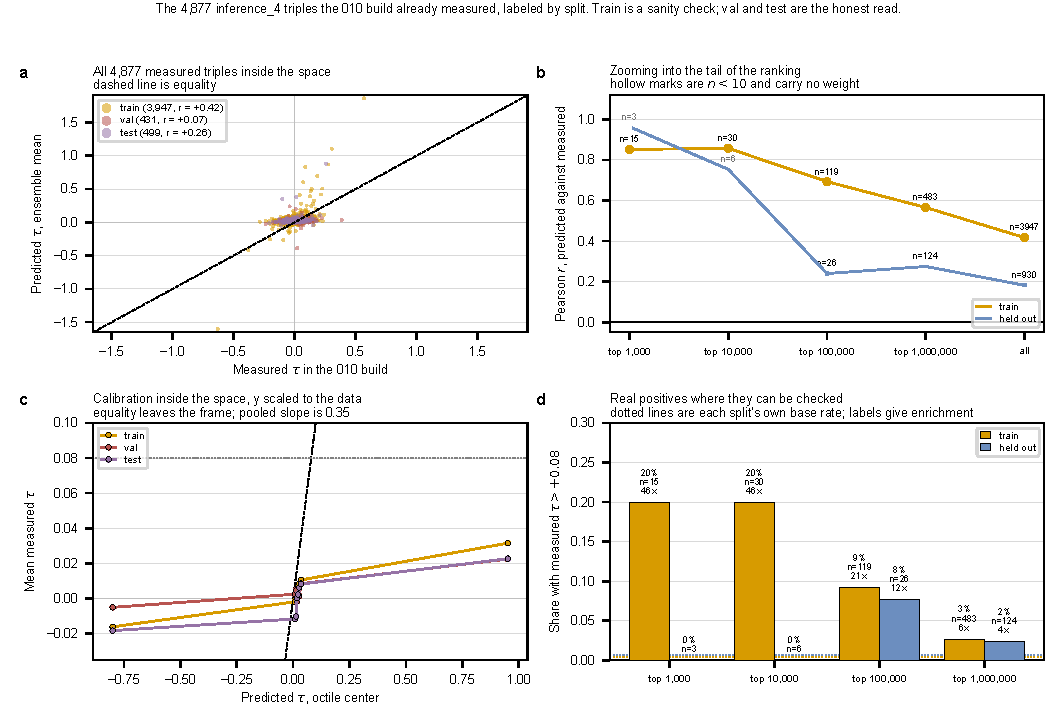
\includegraphics[width=\linewidth]{figures/inference_4_measured_diagnostic.pdf}
\caption{\textbf{a}, predicted against measured $\tau$ for all 4{,}877 measured
triples in the space, by 010 split, with the equality line. \textbf{b}, Pearson $r$
inside rank windows of the ensemble ranking; hollow marks carry fewer than 10
points and are not interpretable. \textbf{c}, mean measured $\tau$ against
predicted octile, with the vertical axis scaled to the measured range, so the
equality line leaves the frame. \textbf{d}, share of measured triples in each
window that are real positive calls, with each split's own base rate dotted and the
enrichment labeled. Generated by
\protect\file{experiments/010-kuzmin-tmi/scripts/inference\_4\_measured\_diagnostic.py}.}
\end{figure}

\subsection{What this panel does not settle\secstatus{todo}}

\pfstep{Whether the effect is the branch point or the regulators} Every triple
carries at least one regulator by construction, \gene{TOS8} in four of the six,
\gene{CAD1} in three and \gene{CUP9} in two, so a regulator-driven result and a
chassis-driven result are separable by the arm contrast and by nothing else in
the design.

\pfstep{Whether growth rescue implies anything about titer} It does not, on this
evidence. The readout is colony growth on rich medium.

\pfstep{Whether the ranking survives a disjoint split} Unchanged from the rest of
this document. The additive null falls from $0.400$ to $0.127 \pm 0.033$ under a
query-pair-disjoint split and the transformer has not been refit there, so every
predicted $\tau$ above is conditional on a split whose leakage is quantified and
whose replacement has not been run.

\pfstep{Whether the axis is the right proxy} Subsystem membership is a
reproducible stand-in for ``genes strain engineering deletes'', and it is not the
same thing. A curated intervention list drawn from the same survey's
gene-level records would be a sharper axis, and it would change which triples are
candidates.

\pfstep{Whether the tail generalizes or only recalls} Partly settled above, and
only partly. The ordering carries held-out signal where measured triples
accumulate, but the window a panel is drawn from holds six of them, so the tail
this panel occupies is not validated by anything in this document.

